\documentclass[11pt,preprint, authoryear]{elsarticle}

\usepackage{lmodern}
%%%% My spacing
\usepackage{setspace}
\setstretch{1.2}
\DeclareMathSizes{12}{14}{10}{10}

% Wrap around which gives all figures included the [H] command, or places it "here". This can be tedious to code in Rmarkdown.
\usepackage{float}
\let\origfigure\figure
\let\endorigfigure\endfigure
\renewenvironment{figure}[1][2] {
    \expandafter\origfigure\expandafter[H]
} {
    \endorigfigure
}

\let\origtable\table
\let\endorigtable\endtable
\renewenvironment{table}[1][2] {
    \expandafter\origtable\expandafter[H]
} {
    \endorigtable
}


\usepackage{ifxetex,ifluatex}
\usepackage{fixltx2e} % provides \textsubscript
\ifnum 0\ifxetex 1\fi\ifluatex 1\fi=0 % if pdftex
  \usepackage[T1]{fontenc}
  \usepackage[utf8]{inputenc}
\else % if luatex or xelatex
  \ifxetex
    \usepackage{mathspec}
    \usepackage{xltxtra,xunicode}
  \else
    \usepackage{fontspec}
  \fi
  \defaultfontfeatures{Mapping=tex-text,Scale=MatchLowercase}
  \newcommand{\euro}{€}
\fi

\usepackage{amssymb, amsmath, amsthm, amsfonts}

\def\bibsection{\section*{References}} %%% Make "References" appear before bibliography


\usepackage[round]{natbib}

\usepackage{longtable}
\usepackage[margin=2.3cm,bottom=2cm,top=2.5cm, includefoot]{geometry}
\usepackage{fancyhdr}
\usepackage[bottom, hang, flushmargin]{footmisc}
\usepackage{graphicx}
\numberwithin{equation}{section}
\numberwithin{figure}{section}
\numberwithin{table}{section}
\setlength{\parindent}{0cm}
\setlength{\parskip}{1.3ex plus 0.5ex minus 0.3ex}
\usepackage{textcomp}
\renewcommand{\headrulewidth}{0.2pt}
\renewcommand{\footrulewidth}{0.3pt}

\usepackage{array}
\newcolumntype{x}[1]{>{\centering\arraybackslash\hspace{0pt}}p{#1}}

%%%%  Remove the "preprint submitted to" part. Don't worry about this either, it just looks better without it:
\makeatletter
\def\ps@pprintTitle{%
  \let\@oddhead\@empty
  \let\@evenhead\@empty
  \let\@oddfoot\@empty
  \let\@evenfoot\@oddfoot
}
\makeatother

 \def\tightlist{} % This allows for subbullets!

\usepackage{hyperref}
\hypersetup{breaklinks=true,
            bookmarks=true,
            colorlinks=true,
            citecolor=blue,
            urlcolor=blue,
            linkcolor=blue,
            pdfborder={0 0 0}}


% The following packages allow huxtable to work:
\usepackage{siunitx}
\usepackage{multirow}
\usepackage{hhline}
\usepackage{calc}
\usepackage{tabularx}
\usepackage{booktabs}
\usepackage{caption}


\newenvironment{columns}[1][]{}{}

\newenvironment{column}[1]{\begin{minipage}{#1}\ignorespaces}{%
\end{minipage}
\ifhmode\unskip\fi
\aftergroup\useignorespacesandallpars}

\def\useignorespacesandallpars#1\ignorespaces\fi{%
#1\fi\ignorespacesandallpars}

\makeatletter
\def\ignorespacesandallpars{%
  \@ifnextchar\par
    {\expandafter\ignorespacesandallpars\@gobble}%
    {}%
}
\makeatother

\newlength{\cslhangindent}
\setlength{\cslhangindent}{1.5em}
\newenvironment{CSLReferences}%
  {\setlength{\parindent}{0pt}%
  \everypar{\setlength{\hangindent}{\cslhangindent}}\ignorespaces}%
  {\par}


\urlstyle{same}  % don't use monospace font for urls
\setlength{\parindent}{0pt}
\setlength{\parskip}{6pt plus 2pt minus 1pt}
\setlength{\emergencystretch}{3em}  % prevent overfull lines
\setcounter{secnumdepth}{5}

%%% Use protect on footnotes to avoid problems with footnotes in titles
\let\rmarkdownfootnote\footnote%
\def\footnote{\protect\rmarkdownfootnote}
\IfFileExists{upquote.sty}{\usepackage{upquote}}{}

%%% Include extra packages specified by user

%%% Hard setting column skips for reports - this ensures greater consistency and control over the length settings in the document.
%% page layout
%% paragraphs
\setlength{\baselineskip}{12pt plus 0pt minus 0pt}
\setlength{\parskip}{12pt plus 0pt minus 0pt}
\setlength{\parindent}{0pt plus 0pt minus 0pt}
%% floats
\setlength{\floatsep}{12pt plus 0 pt minus 0pt}
\setlength{\textfloatsep}{20pt plus 0pt minus 0pt}
\setlength{\intextsep}{14pt plus 0pt minus 0pt}
\setlength{\dbltextfloatsep}{20pt plus 0pt minus 0pt}
\setlength{\dblfloatsep}{14pt plus 0pt minus 0pt}
%% maths
\setlength{\abovedisplayskip}{12pt plus 0pt minus 0pt}
\setlength{\belowdisplayskip}{12pt plus 0pt minus 0pt}
%% lists
\setlength{\topsep}{10pt plus 0pt minus 0pt}
\setlength{\partopsep}{3pt plus 0pt minus 0pt}
\setlength{\itemsep}{5pt plus 0pt minus 0pt}
\setlength{\labelsep}{8mm plus 0mm minus 0mm}
\setlength{\parsep}{\the\parskip}
\setlength{\listparindent}{\the\parindent}
%% verbatim
\setlength{\fboxsep}{5pt plus 0pt minus 0pt}



\begin{document}



\begin{frontmatter}  %

\title{A Replication: Identifying Aggregate Supply and Demand Shocks in
SouthAfrica}

% Set to FALSE if wanting to remove title (for submission)




\author[Add1]{Samantha Scott}
\ead{20945043@sun.ac.za}





\address[Add1]{Stellenbosch University, Cape Town, South Africa}



\vspace{1cm}


\begin{keyword}
\footnotesize{
Econometrics \sep Time Series \sep VAR \sep SVAR \sep Blanchard-Quah \\
\vspace{0.3cm}
}
\end{keyword}



\vspace{0.5cm}

\end{frontmatter}


\renewcommand{\contentsname}{Table of Contents}
{\tableofcontents}

%________________________
% Header and Footers
%%%%%%%%%%%%%%%%%%%%%%%%%%%%%%%%%
\pagestyle{fancy}
\chead{}
\rhead{Innovation Accounting Replication and Robustness Checks}
\lfoot{}
\rfoot{\footnotesize Page \thepage}
\lhead{}
%\rfoot{\footnotesize Page \thepage } % "e.g. Page 2"
\cfoot{}

%\setlength\headheight{30pt}
%%%%%%%%%%%%%%%%%%%%%%%%%%%%%%%%%
%________________________

\headsep 35pt % So that header does not go over title




\newpage

\newpage

\hypertarget{introduction}{%
\section{Introduction}\label{introduction}}

The paper \emph{Identifying aggregate supply and demand shocks in South
Africa} is an application of a structural VAR method to identify supply
and demand shocks for the South African economy since the 1960s. The aim
of this investigation is to replicate the innovation accounting
presented by Du Plessis, Smit and Sturzenegger (2007), with additional
robustness checks. Using data found from an alternative source, it is
evident that the model does not present the same results as the impulse
response functions are significantly different to that of the original
paper. As such, the results of this paper are not consistent with
theoretical priors presented by Du Plessis, Smit and Sturzenegger
(2007).

After conducting several robustness checks, it is clear that the
residuals of two of the main variables, namely the government
consumption to GDP ratio as well as the real interest rate, are not
white noise. It is also made evident that seasonally adjusting the real
interest rate and differencing the variable by one to achieve
stationarity significantly impacted the results of the model.

\hypertarget{data}{%
\section{Data}\label{data}}

The data used is quarterly data from FRED, dating back to the second
quarter of 1960 up until 2007. Similarly to the original paper, a
robustness check is conducted using a shorter sample is used from the
fourth quarter of 1983. Unlike the original paper, the data used is not
seasonally adjusted. The variables used in the model are the first
difference of the log of real GDP (\(y_t\)), the ratio of government
consumption to GDP (\(g_t\)), as well the real interest rate (\(r_t\)).
\(r_t\) is calculated using the monthly nominal interest rate as well as
the monthly CPI data. Below is the equation used to calculate \(r_t\).

\[ r_t = ((1 + Avg(i_{mt-1}, i_{mt}, i_{mt+1}))/(1+(ln(CPI_{mt-2}) - ln(CPI_{mt+1}))) ^ 4 - 1)*100 \]
Figures 1, 2 and 3 represent the variables used in the model. As seen in
the Appendix, when an Augmented Dickey-Fuller test is conducted, it is
evident that \(y_t\) is stationary, as the p-value is less than 0.05.
However, both \(g_t\) and \(r_t\) are non-stationary. In the original
paper (2007), \(r_t\) is stationary. To test the impact of the
difference between the \(r_t\) variables, a robustness check is
conducted where the real interest rate is seasonally adjusted and made
stationary.

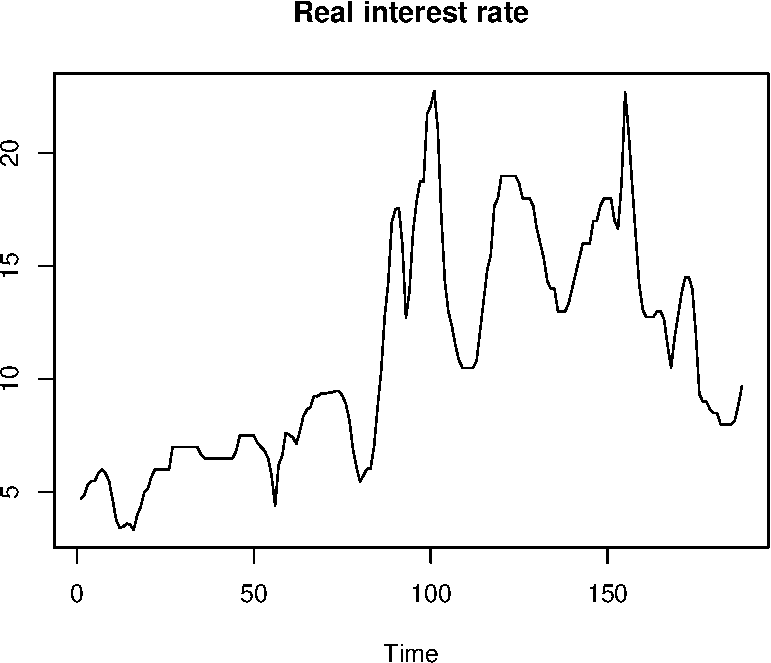
\includegraphics{TS_proj_files/figure-latex/unnamed-chunk-12-1.pdf}

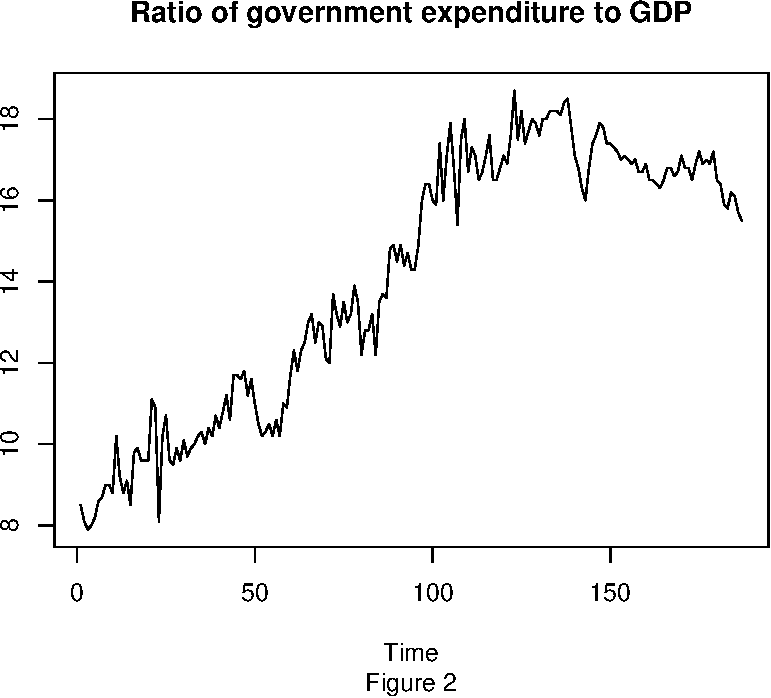
\includegraphics{TS_proj_files/figure-latex/unnamed-chunk-13-1.pdf}

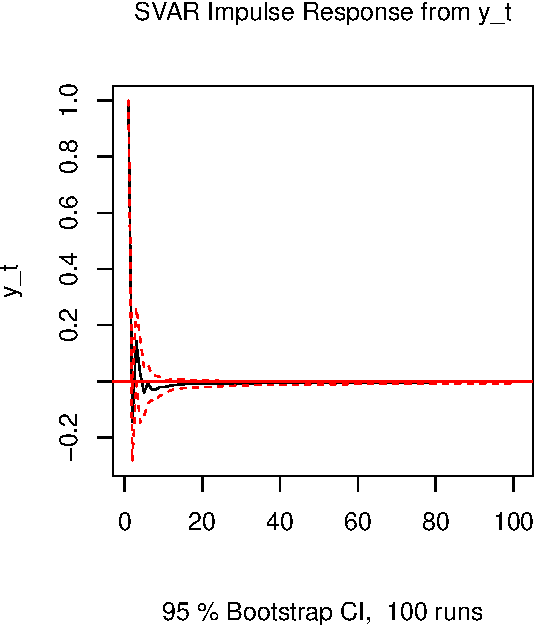
\includegraphics{TS_proj_files/figure-latex/unnamed-chunk-14-1.pdf}

\hypertarget{methodology}{%
\section{Methodology}\label{methodology}}

A structural VAR model is created to identify supply and demand shocks
for the South African economy since the 1960s. The demand the variables,
\(y_t\), \(g_t\) and \(r_t\) are proxies for a supply shock, a fiscal
shock and a monetary shock, respectively. In the three variable model,
Du Plessis, Smit and Sturzenegger (2007) present three restrictions
necessary to identify the structural shocks and the dynamics of the
structural system. The first two restrictions require that fiscal and
monetary policy shocks have no long-run effects on real GDP. The final
restriction in that the long run effect of monetary policy on the stance
of fiscal policy is also restricted to zero. These restrictions create a
lower-triangular matrix, which is replicated for this investigation. The
reduced form VAR in this investigation was estimated with three lags.
The original paper (2007), conducted the estimation using four lags. The
results of the SVAR model are presented as impulse response functions,
as well as through a variance decomposition.

\hypertarget{results}{%
\section{Results}\label{results}}

This section is a discussion of the results, as well as a comparison to
those of Du Plessis, Smit and Sturzenegger (2007). The authors make use
of innovation accounting, which entails the consideration of the impulse
response and variance decomposition of SVAR models. The first step of
innovation accounting is to inspect the impulse response functions of
the identified shocks to determine whether they match theoretical priors
about discretion and magnitude of impact. The results of the model using
the longer dataset (1960+) are presented as impulse response functions
in the subsections below.

\hypertarget{impulse-response-of-real-gdp-for-each-of-the-identified-shocks}{%
\subsection{Impulse Response of real GDP for each of the identified
shocks}\label{impulse-response-of-real-gdp-for-each-of-the-identified-shocks}}

In the original paper (2007), the impulse response functions of real GDP
for each of the identified shocks are consistent with theoretical
priors. The supply shock has a permanent impact on real GDP, while the
demand shocks have transitionary impacts. In opposition, the results of
this paper indicates that the the supply shock has a transitory impact
while the demand shocks have permanent, negative impacts on real GDP.

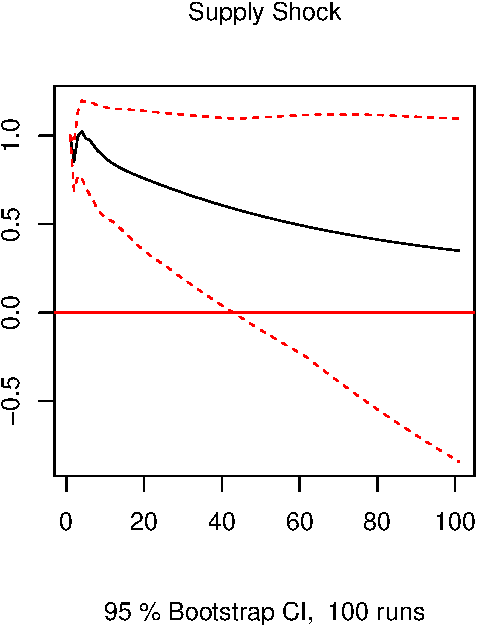
\includegraphics{TS_proj_files/figure-latex/unnamed-chunk-18-1.pdf}
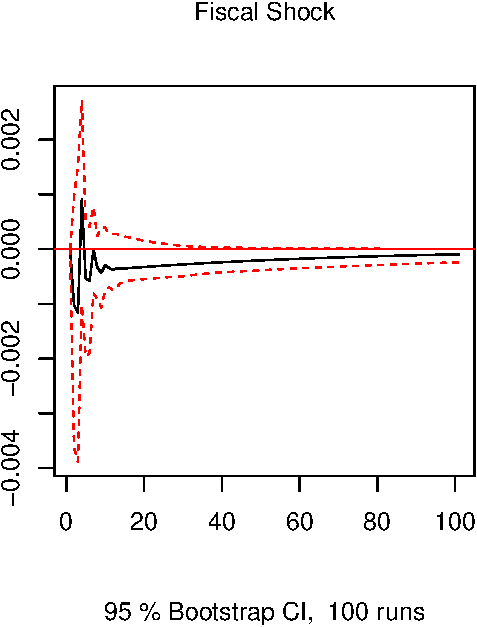
\includegraphics{TS_proj_files/figure-latex/unnamed-chunk-18-2.pdf}
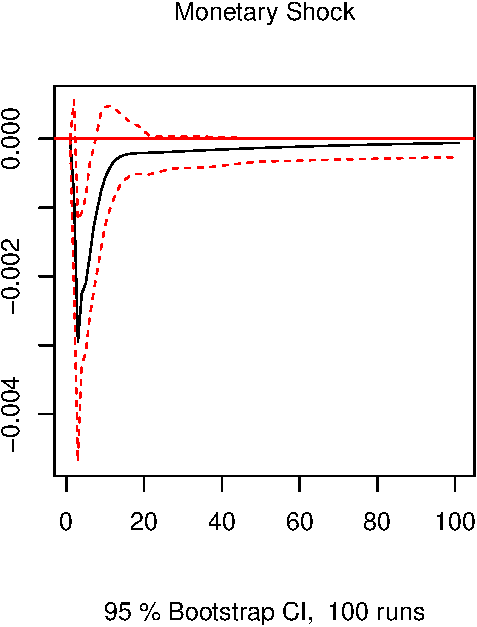
\includegraphics{TS_proj_files/figure-latex/unnamed-chunk-18-3.pdf}

\newpage

\hypertarget{impulse-response-of-the-real-interest-rate-for-each-of-the-identified-shocks}{%
\subsection{Impulse Response of the real interest rate for each of the
identified
shocks}\label{impulse-response-of-the-real-interest-rate-for-each-of-the-identified-shocks}}

The impulse response functions in the original paper suggest that a
positive supply shock raises the real interest rate temporarily. This is
also indicated in the results of this investigation, however, the real
interest rate is slower to respond to the rise in the supply shock than
in the original paper. Du Plessis, Smit and Sturzenegger (2007) find
that positive fiscal shock lowers the real interest rate temporarily,
which indicates that a fiscal stimulus is met with accomodating monetary
policy. However, this is not the result of this investigation. As
indicated below, a positive fiscal shock results in a an increase in the
real interest rate, which is slow to respond.

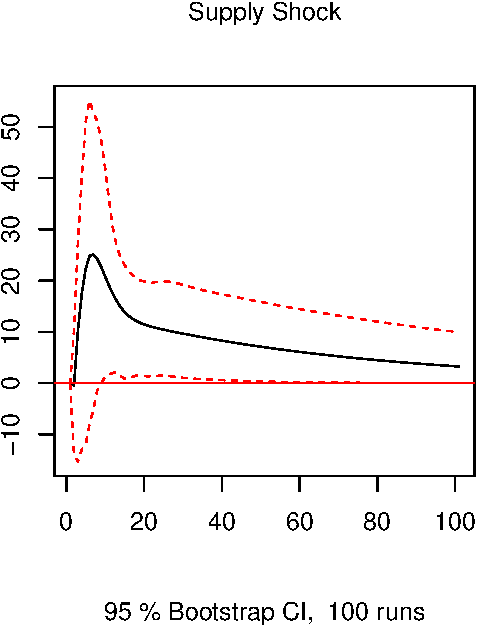
\includegraphics{TS_proj_files/figure-latex/unnamed-chunk-19-1.pdf}
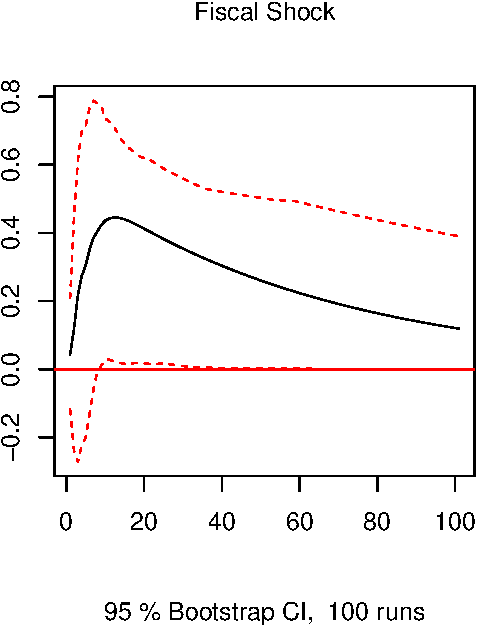
\includegraphics{TS_proj_files/figure-latex/unnamed-chunk-19-2.pdf}
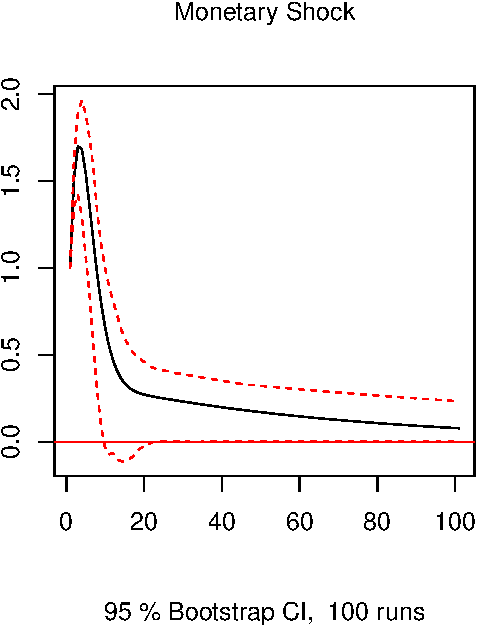
\includegraphics{TS_proj_files/figure-latex/unnamed-chunk-19-3.pdf}

\newpage

\hypertarget{impulse-response-of-the-government-consumption-to-real-gdp-for-each-of-the-identified-shocks}{%
\subsection{Impulse Response of the government consumption to real GDP
for each of the identified
shocks}\label{impulse-response-of-the-government-consumption-to-real-gdp-for-each-of-the-identified-shocks}}

Du Plessis, Smit and Sturzenegger (2007)'s results find that GDP
responds faster to a positive supply shock than government expenditure.
The results of this investigative present a similar result, as indicated
in the impulse response functions below. However, a positive supply
shock results in government expenditure to fall below zero before moving
back towards zero. The impulse response functions of the investigation
indicate that a positive supply shock results in government expenditure
to rise before moving back to zero.

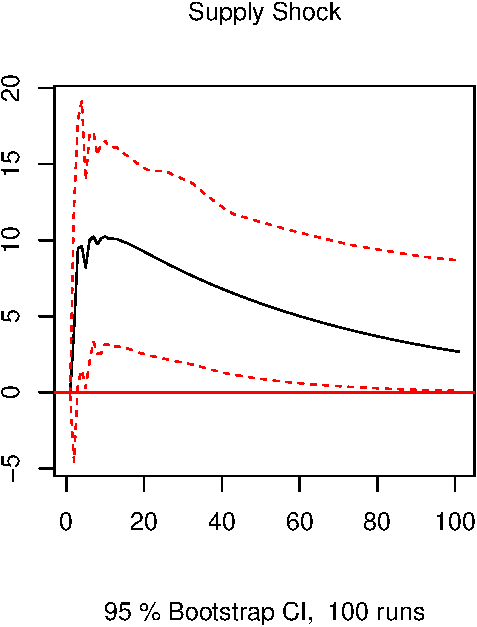
\includegraphics{TS_proj_files/figure-latex/unnamed-chunk-20-1.pdf}
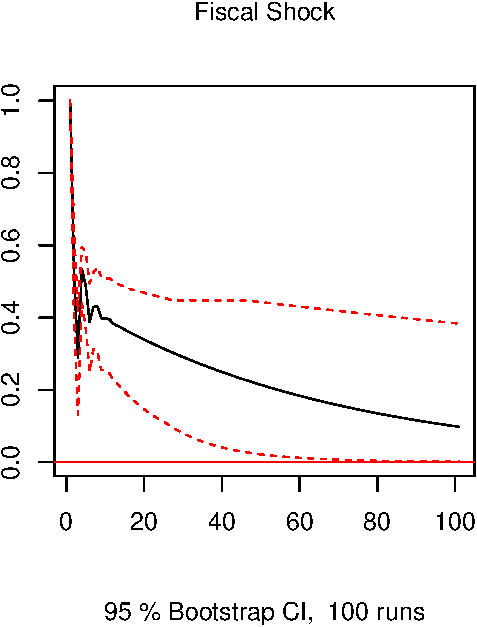
\includegraphics{TS_proj_files/figure-latex/unnamed-chunk-20-2.pdf}
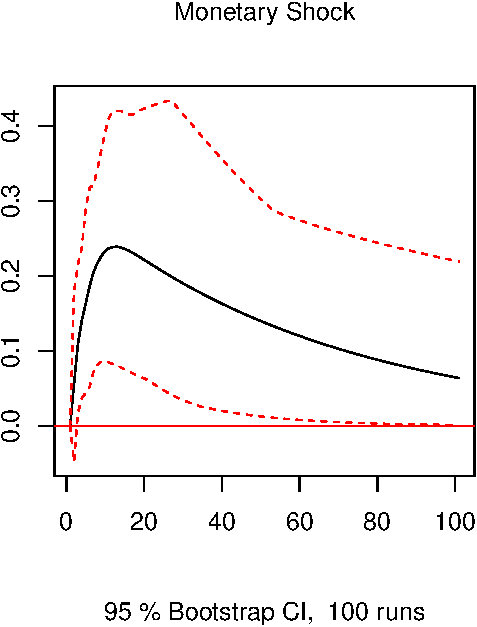
\includegraphics{TS_proj_files/figure-latex/unnamed-chunk-20-3.pdf}

\newpage

\hypertarget{variance-decomposition}{%
\subsection{Variance Decomposition}\label{variance-decomposition}}

A variance decomposition indicates the amount of information that each
variable contributes to the other variables in the model. The variance
decomposition therefore determines how much of the forecast error
variance of each of the variables can be explained by exogenous shocks
to the other variables (Lütkepohl, 2010).

The variance decomposition of real GDP shows the proportion of the
variance of real GDP which can be accounted for by the three identified
shocks over various horizons. The first plot below is the variance
decomposition of real GDP for the longer sample. The second plot
presents the variance decomposition of real GDP for a shorter sample. In
the larger sample, both \(g_t\) and \(r_t\) are initially dependent on
the value they are set to be. However, as time passes, it is evident
that \(g_t\) and \(r_t\) are impacted by \(y_t\).

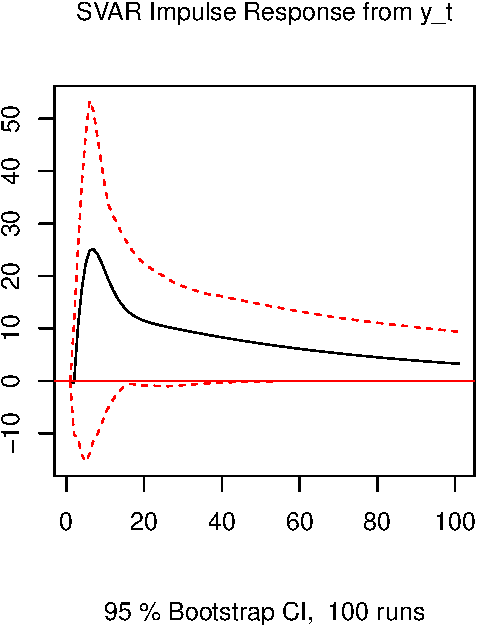
\includegraphics{TS_proj_files/figure-latex/unnamed-chunk-21-1.pdf}

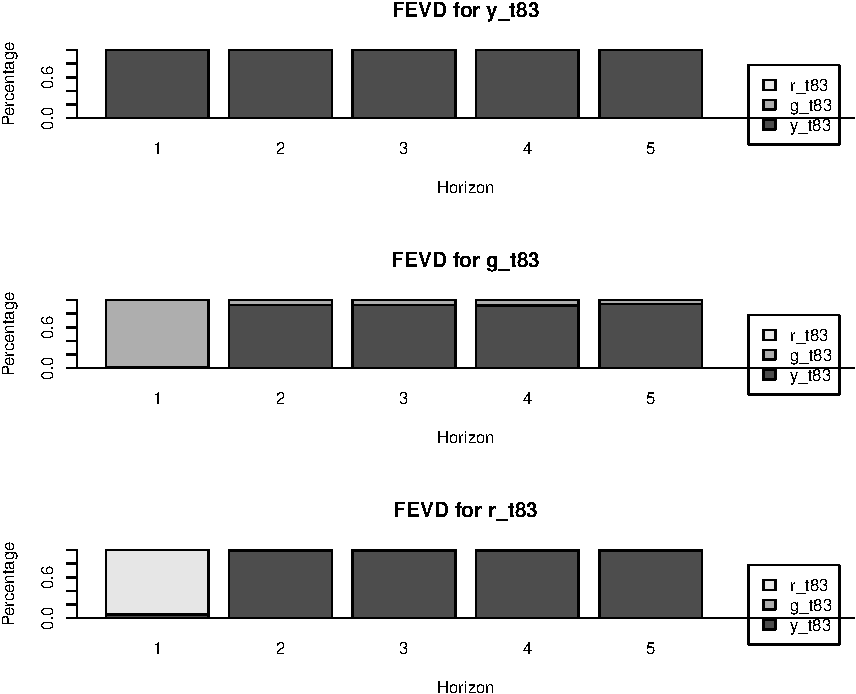
\includegraphics{TS_proj_files/figure-latex/unnamed-chunk-22-1.pdf}

\hypertarget{robustness-checks}{%
\section{Robustness Checks}\label{robustness-checks}}

In this section, four robustness checks are conducted to test whether
estimated effects of interest are sensitive to changes in model
specifications. First, the real interest rate variable (\(r_t\)) is
manually seasonally adjusted, and made stationary. Second, the residuals
of the time series variables are investiagted in order to determine if
they are white noise. Third, the number of lags specified in the model
is altered. Lastly, a reduced sample (from the fourth quarter of 1983)
is used in place of the larger sample.

\hypertarget{removing-seasonality}{%
\subsection{Removing Seasonality}\label{removing-seasonality}}

For the last robustness check, the data used to calculate the real
interest rate is seasonally adjusted. Further, the real interest rate
data is differenced by 1, resulting in a stationary time series. As seen
in the Appendix, the new, seasonally adjusted data that is differenced
by 1 is stationary, with a p-value of 0.01 when an Aumented
Dickey-Fuller test is conducted. The new real interest rate variable is
depicted below:

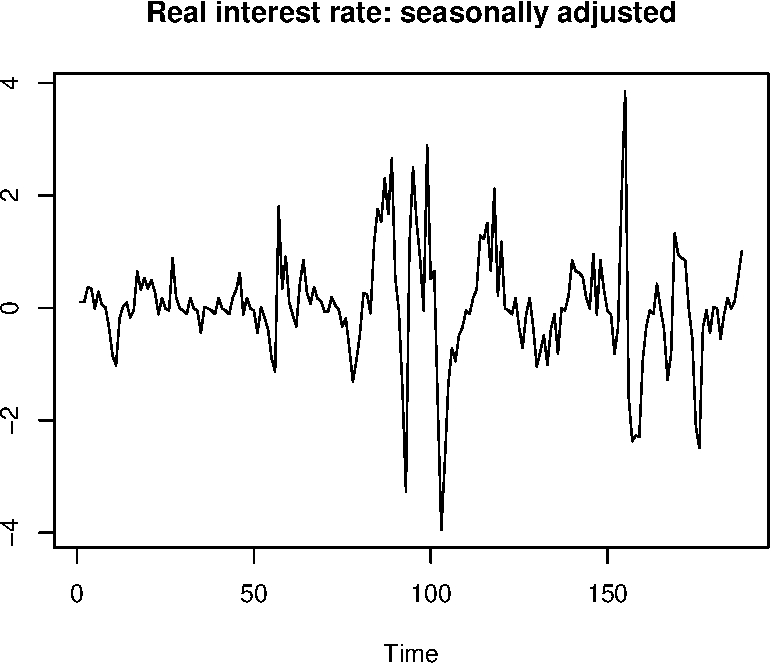
\includegraphics{TS_proj_files/figure-latex/unnamed-chunk-23-1.pdf}

As depicted by the impulse response function of the real interest rate
for each of the identified shocks in the Appendix, the method of
removing seasonality and making the variable \(r_t\) stationary, the new
impulse response functions are more comparable to those of the original
paper than previosuly. This indicates that removing seasonality from the
main variables is essential.

\hypertarget{residuals}{%
\subsection{Residuals}\label{residuals}}

As the next robustness check, the residuals of the variables \(y_t\),
\(g_t\), \(r_t\), as well as the seasonally adjusted, normalised real
interest rate variable are investigated in order to determine whether
their respective residuals are white noise. White noise is defined as a
time series that is purely random. The residuals are defined as the
difference between the fitted model and the data. If the model is a good
fit, the residuals should be white noise.

\newpage

Below is the result of a check for residuals for the \(y_t\) variable.
As indicated by the figures, the residuals of \(y_t\) are white noise.
The residuals are random, with no apparent trend. However, the
autocorrelation in the second and third lags are significantly larger
than zero. When conducting a Ljung\_Box test, the p-value in greater
that 0.01. As such we cannot reject the null hypothesis, indicating that
the time series does not contain an autocorrelation.

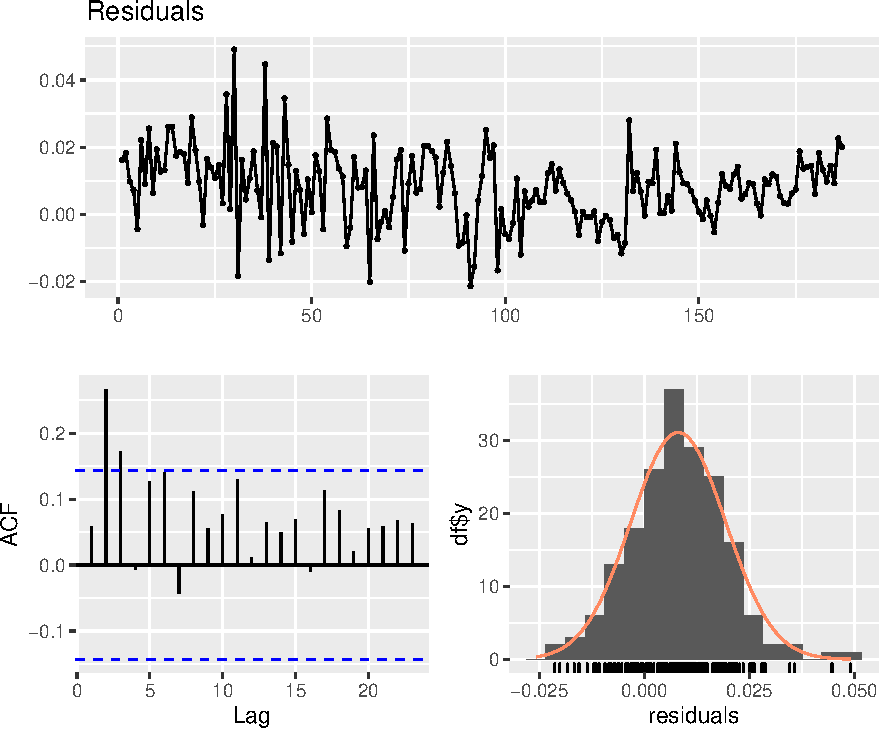
\includegraphics{TS_proj_files/figure-latex/unnamed-chunk-24-1.pdf}

\newpage

The figures below indicate that the residuals for the \(g_t\) variable
are not white noise. When conducting a Ljung-Box test, the p-value is
smaller than 0.01, thus we can reject the null hypothesis. Therefore,
the time series does contain an autocorrelation and the residuals are
not white noise.

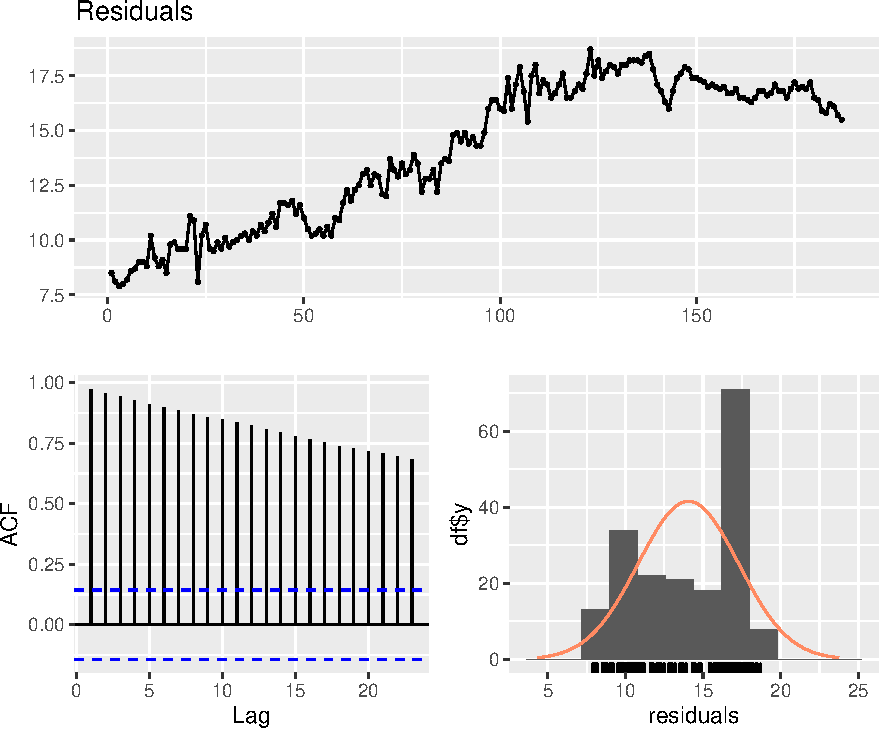
\includegraphics{TS_proj_files/figure-latex/unnamed-chunk-25-1.pdf}

\newpage

The figures below are checks for residuals for the \(r_t\) variable. The
figures indicate that the residuals are not white noise. The
autocorrelation in all of the lags are larger than zero. The Ljung-Box
test indicates that there is correlation in the time series, as the
p-value is lower than 0.01.

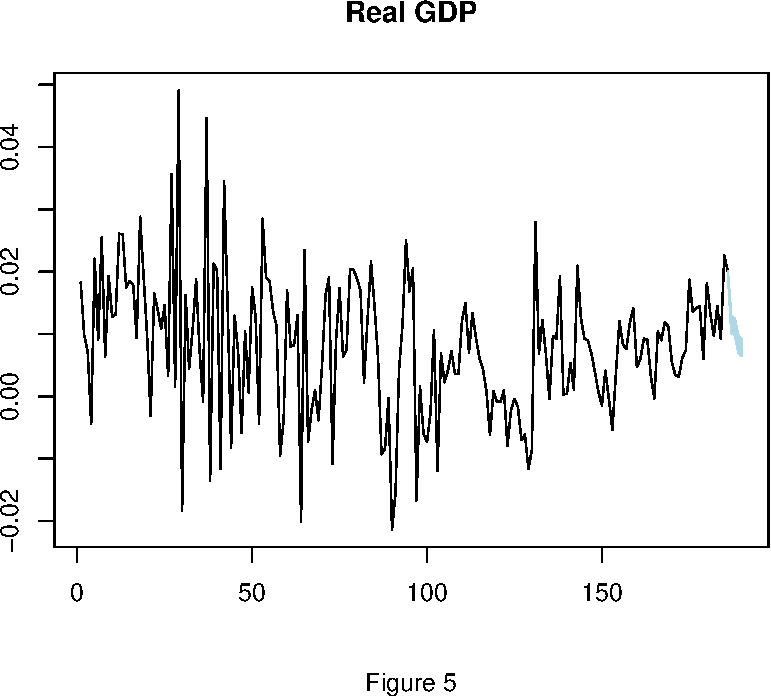
\includegraphics{TS_proj_files/figure-latex/unnamed-chunk-26-1.pdf}

\newpage

The figures below present a check for residuals for an interest rate
variable that has been seasonally adjusted and made stationary. The
residuals seem to be random, without an apparent trend. The
autocorrelation in the first two lags are greater than zero. When
conducting a Ljung-Box test, the p-value is less than 0.01. As such, we
can reject the null hypothesis. Therefore, the time series contains
autocorrelation, and the residuals are not white noise.

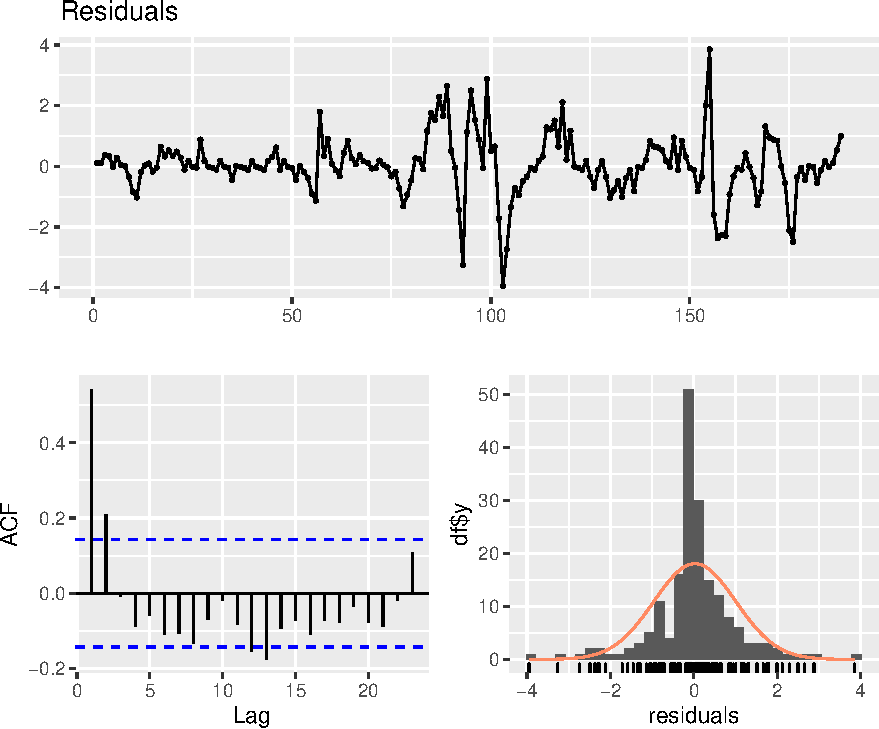
\includegraphics{TS_proj_files/figure-latex/unnamed-chunk-27-1.pdf}

\newpage

\hypertarget{lag-selection}{%
\subsection{Lag Selection}\label{lag-selection}}

According to Ozcicek and Mcmillin (1999:517-518), overfitting, which
entails selecting a higher order lag length than the true lag length,
causes an increase in the mean-square forecast errors of the VAR.
Underfitting the lag length results in autocorrelated errors. As such,
it is important to test whether the number of lags selected may
influence the results of the model.

As another robustness check, additional models are generated with more
and less variables than the initial model. First, a model with more lags
(6) than the selected amount (3), and second, less lags (2) than the lag
order selection number. As seen by the impulse response functions of
these additional models, the results were not greatly impacted by a
change in the number of lags.

\hypertarget{reduced-sample}{%
\subsection{Reduced Sample}\label{reduced-sample}}

As another robustness check, a smaller sample is used, dating from the
fourth quarter of 1963 to the last quarter of 2006. The same method is
applied to assess whether the sample selected may alter the results. As
seen by the impulse response functions in the Appendix, using a smaller
sample (1983+) does not significantly impact the results, as they are
comparable to the impulse response functions of the larger sample
(1960+).

\hypertarget{conclusion}{%
\section{Conclusion}\label{conclusion}}

This investigation served as an attempt to replicate the innovation
accounting in Du Plessis, Smit and Sturzenegger (2007)'s paper, using
data from an alternative source. A structural VAR method was applied to
identify aggregate supply and aggregate demand shocks for the South
African economy from the 1960s. The impulse response functions of this
investigation differed from those of the original paper, resulting in
the functions being inconsistent with theory. Additional robustness
checks were conducted, for example a residual check, which revealed that
two of the three main variables used in the model contain residuals that
are not white noise. Other robustness checks altering lag selection, as
well as reducing the sample, indicated that model specifications did not
impact the results of the model. However, by altering the real interest
rate for the variable to be seasonally adjusted and stationary the
impulse response functions were impacted significantly.

\newpage

\hypertarget{reference-list}{%
\section{Reference List}\label{reference-list}}

Du Plessis, S., Smit, B. and Sturzenegger, F., 2007. Identifying
aggregate supply and demand shocks in South Africa. Journal of African
economies, 17(5):765-793.

Lütkepohl, H. 2010. Variance Decomposition. In: Durlauf, S.N., Blume,
L.E. (eds) Macroeconometrics and Time Series Analysis. The New Palgrave
Economics Collection. Palgrave Macmillan, London.

Ozcicek, O \& McMillin, W. D. 1999. Lag Length Selection in Vector
Autoregressive Models: Symmetric and Asymmetric Lags. \emph{Applied
Economics}, 31(4):517-524.

\newpage

\hypertarget{appendix}{%
\section{Appendix}\label{appendix}}

\hypertarget{forecast}{%
\subsection{Forecast}\label{forecast}}

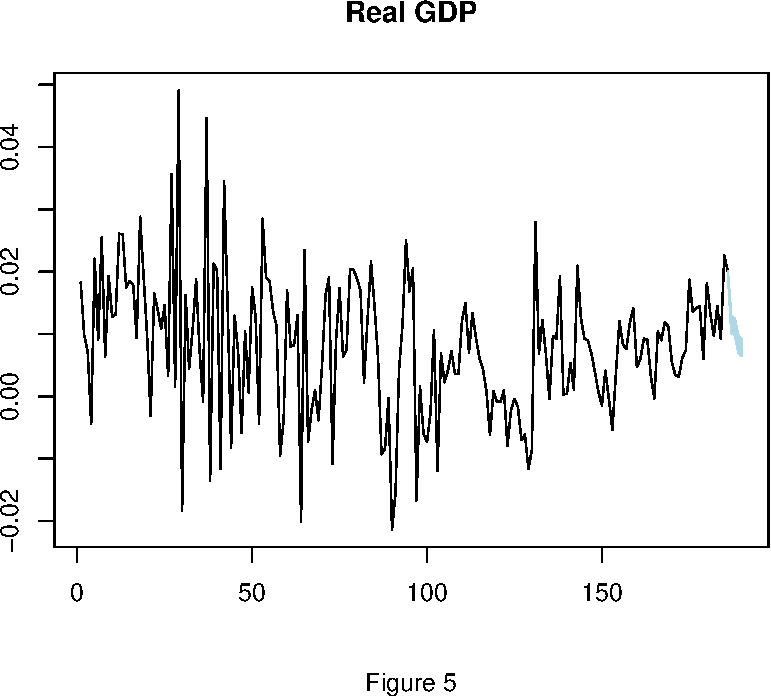
\includegraphics{TS_proj_files/figure-latex/unnamed-chunk-28-1.pdf}

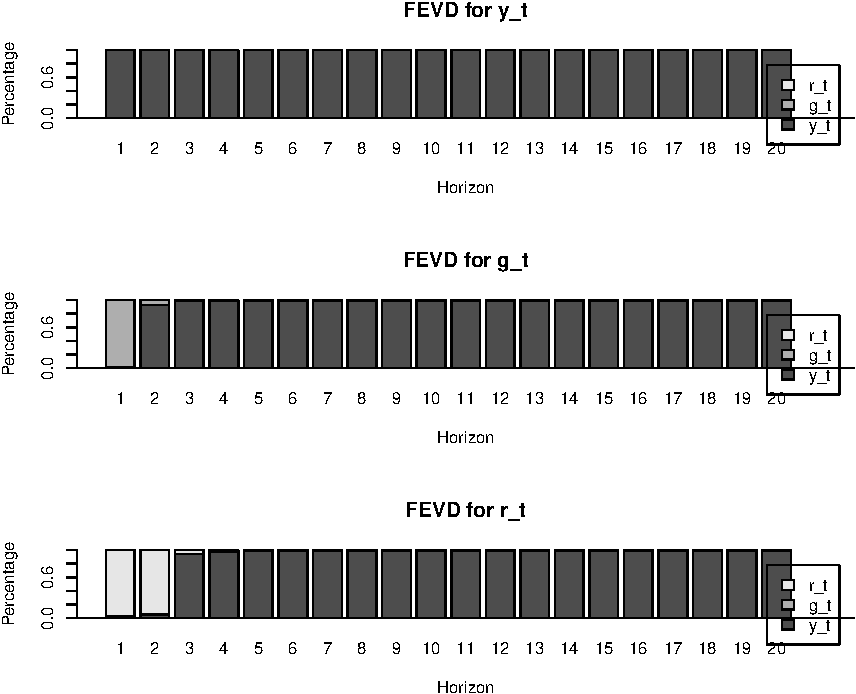
\includegraphics{TS_proj_files/figure-latex/unnamed-chunk-29-1.pdf}

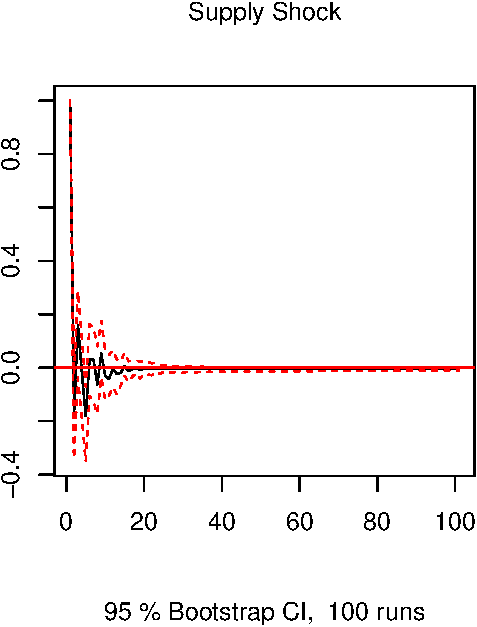
\includegraphics{TS_proj_files/figure-latex/unnamed-chunk-30-1.pdf}

\hypertarget{testing-for-stationarity}{%
\subsection{Testing for Stationarity}\label{testing-for-stationarity}}

\begin{verbatim}
## 
##  Augmented Dickey-Fuller Test
## 
## data:  real_gdp1
## Dickey-Fuller = -3.7922, Lag order = 5, p-value = 0.0208
## alternative hypothesis: stationary
\end{verbatim}

\begin{verbatim}
## 
##  Augmented Dickey-Fuller Test
## 
## data:  rg83
## Dickey-Fuller = -3.5737, Lag order = 4, p-value = 0.03979
## alternative hypothesis: stationary
\end{verbatim}

\begin{verbatim}
## 
##  Augmented Dickey-Fuller Test
## 
## data:  Real_interest1$Real_interest_rate
## Dickey-Fuller = -2.6335, Lag order = 5, p-value = 0.3112
## alternative hypothesis: stationary
\end{verbatim}

\begin{verbatim}
## 
##  Augmented Dickey-Fuller Test
## 
## data:  ri83$Real_interest_rate
## Dickey-Fuller = -2.7977, Lag order = 4, p-value = 0.2473
## alternative hypothesis: stationary
\end{verbatim}

\begin{verbatim}
## 
##  Augmented Dickey-Fuller Test
## 
## data:  ri_sa$seasonally_differenced
## Dickey-Fuller = -5.7783, Lag order = 5, p-value = 0.01
## alternative hypothesis: stationary
\end{verbatim}

\begin{verbatim}
## 
##  Augmented Dickey-Fuller Test
## 
## data:  g_g_not_s$Value
## Dickey-Fuller = -0.66065, Lag order = 5, p-value = 0.9724
## alternative hypothesis: stationary
\end{verbatim}

\begin{verbatim}
## 
##  Augmented Dickey-Fuller Test
## 
## data:  gg83$Value
## Dickey-Fuller = -2.3567, Lag order = 4, p-value = 0.4292
## alternative hypothesis: stationary
\end{verbatim}

\hypertarget{ljung-box-tests}{%
\subsection{Ljung-Box Tests}\label{ljung-box-tests}}

\begin{verbatim}
## 
##  Box-Ljung test
## 
## data:  y_t
## X-squared = 0.63753, df = 1, p-value = 0.4246
\end{verbatim}

\begin{verbatim}
## 
##  Box-Ljung test
## 
## data:  g_t
## X-squared = 179.82, df = 1, p-value < 2.2e-16
\end{verbatim}

\begin{verbatim}
## 
##  Box-Ljung test
## 
## data:  r_t
## X-squared = 181.77, df = 1, p-value < 2.2e-16
\end{verbatim}

\begin{verbatim}
## 
##  Box-Ljung test
## 
## data:  r_t_sa
## X-squared = 56.161, df = 1, p-value = 6.672e-14
\end{verbatim}

\newpage

\hypertarget{removing-seasonality-and-non-stationarity-impulse-response-functions}{%
\subsection{Removing Seasonality and Non-stationarity Impulse Response
Functions}\label{removing-seasonality-and-non-stationarity-impulse-response-functions}}

Impulse Response of real GDP for each of the identified shocks:

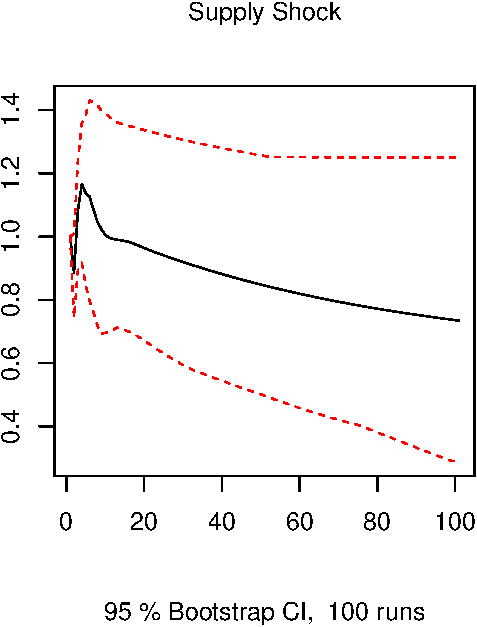
\includegraphics{TS_proj_files/figure-latex/unnamed-chunk-36-1.pdf}
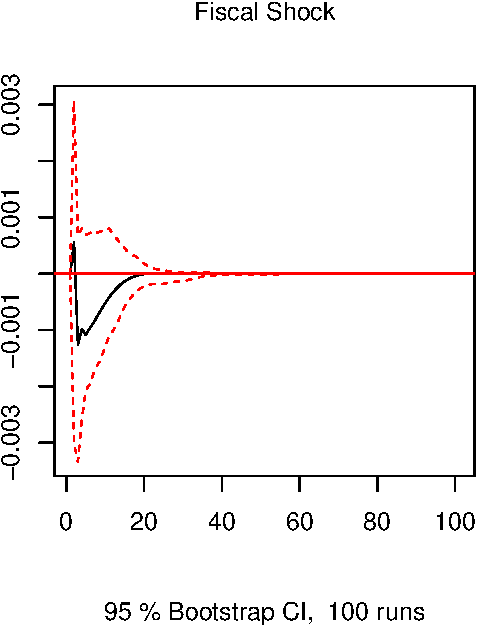
\includegraphics{TS_proj_files/figure-latex/unnamed-chunk-36-2.pdf}
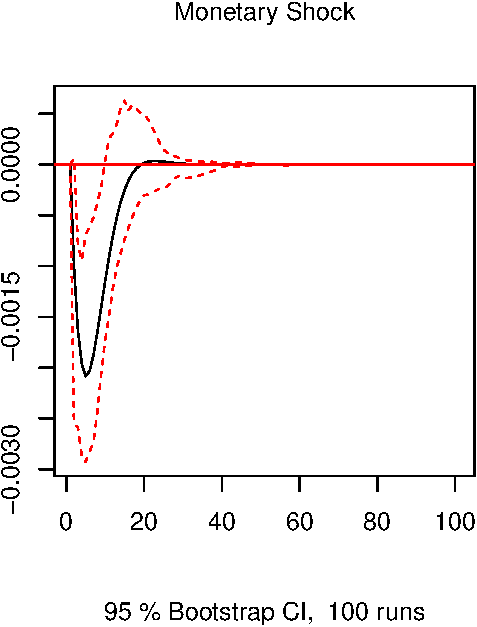
\includegraphics{TS_proj_files/figure-latex/unnamed-chunk-36-3.pdf}
\newpage Impulse Response of the real interest rate for each of the
identified shocks:

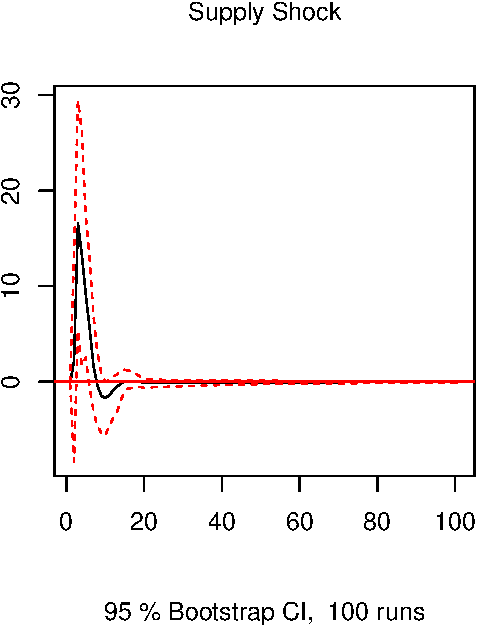
\includegraphics{TS_proj_files/figure-latex/unnamed-chunk-37-1.pdf}
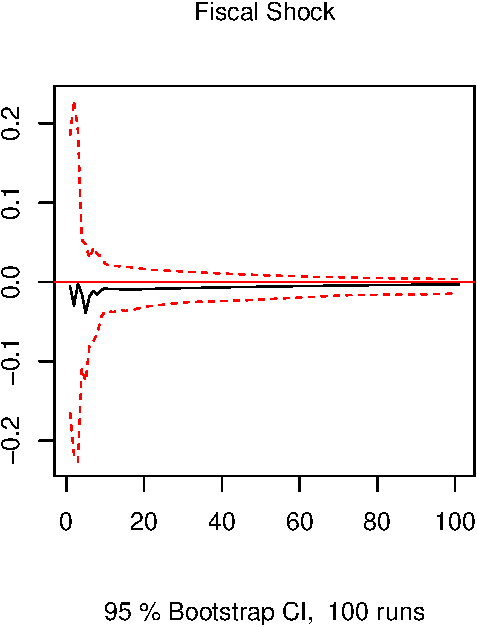
\includegraphics{TS_proj_files/figure-latex/unnamed-chunk-37-2.pdf}
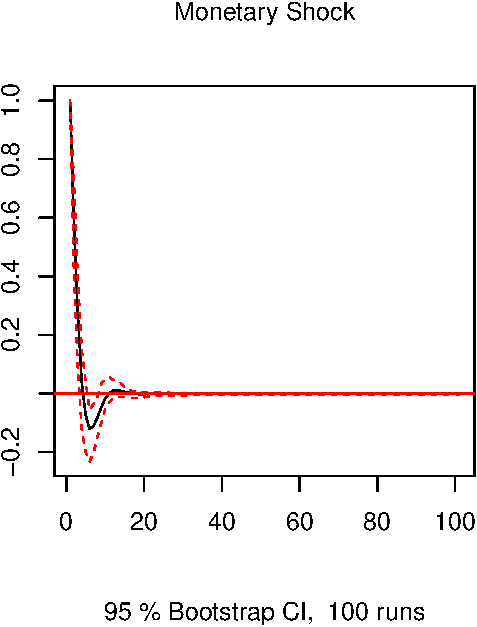
\includegraphics{TS_proj_files/figure-latex/unnamed-chunk-37-3.pdf}
\newpage Impulse Response of the government consumption to real GDP for
each of the identified shocks:

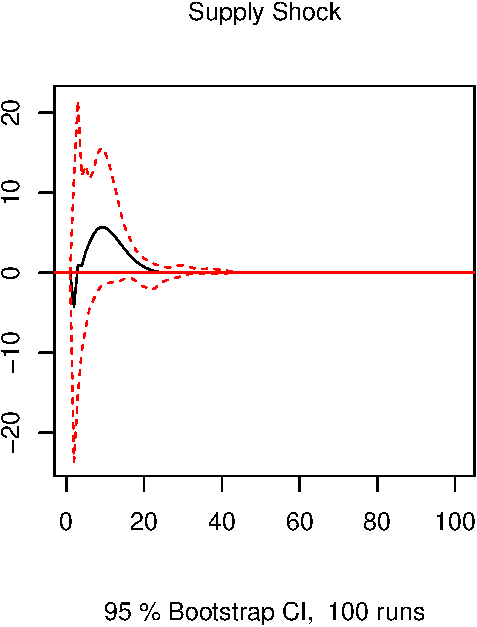
\includegraphics{TS_proj_files/figure-latex/unnamed-chunk-38-1.pdf}
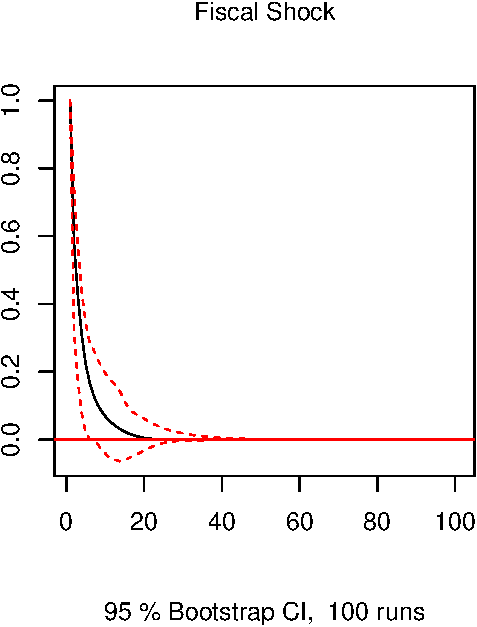
\includegraphics{TS_proj_files/figure-latex/unnamed-chunk-38-2.pdf}
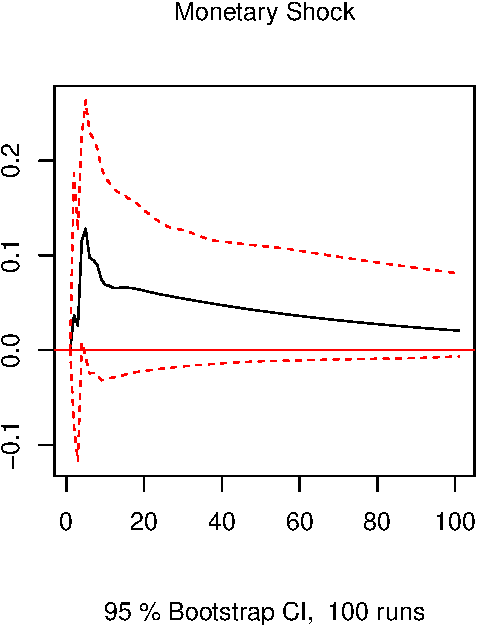
\includegraphics{TS_proj_files/figure-latex/unnamed-chunk-38-3.pdf}

\newpage

\hypertarget{lag-selection-impulse-response-functions}{%
\subsection{Lag Selection Impulse Response
Functions}\label{lag-selection-impulse-response-functions}}

Impulse Response of the real GDP for each of the identified shocks:

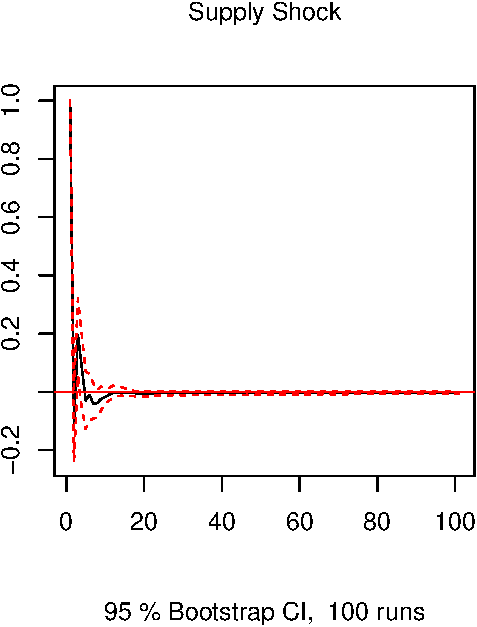
\includegraphics{TS_proj_files/figure-latex/unnamed-chunk-39-1.pdf}
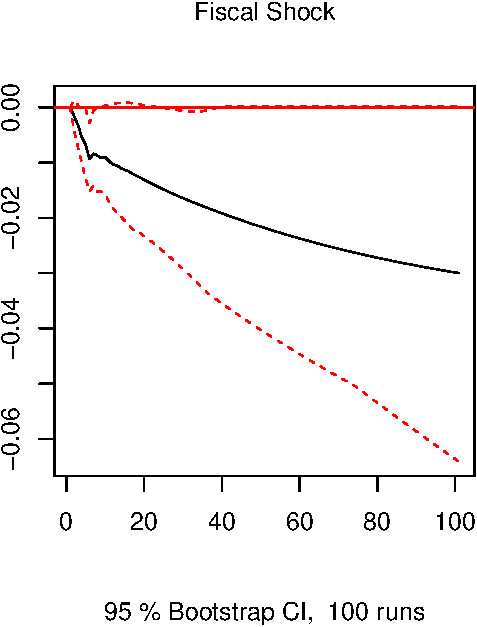
\includegraphics{TS_proj_files/figure-latex/unnamed-chunk-39-2.pdf}
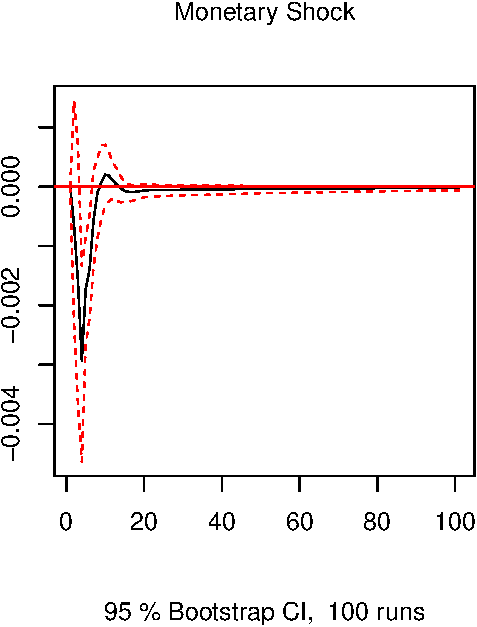
\includegraphics{TS_proj_files/figure-latex/unnamed-chunk-39-3.pdf}

\newpage

Impulse Response of the real interest rate for each of the identified
shocks:

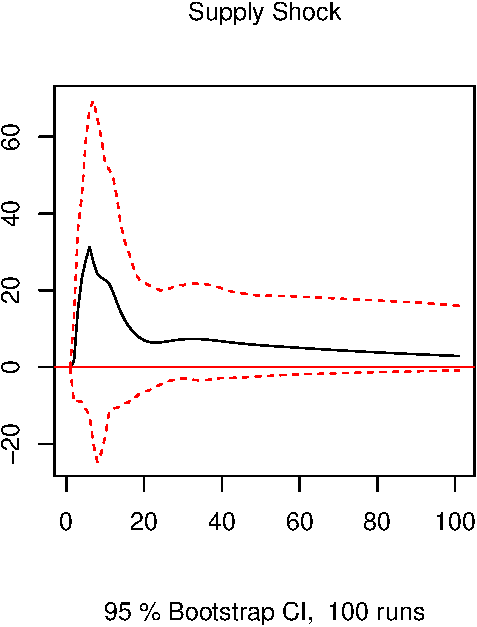
\includegraphics{TS_proj_files/figure-latex/unnamed-chunk-40-1.pdf}
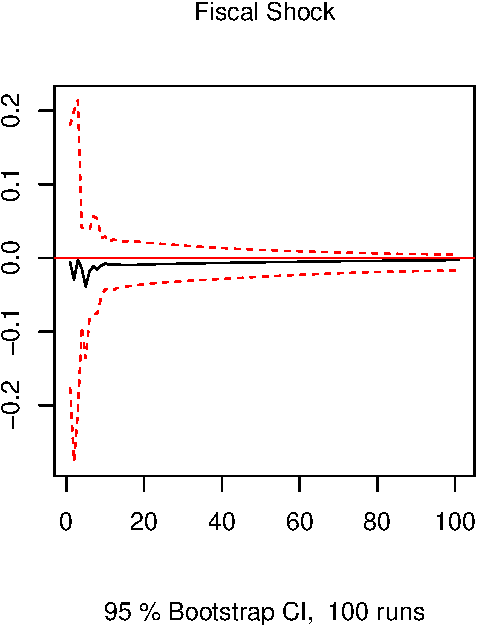
\includegraphics{TS_proj_files/figure-latex/unnamed-chunk-40-2.pdf}
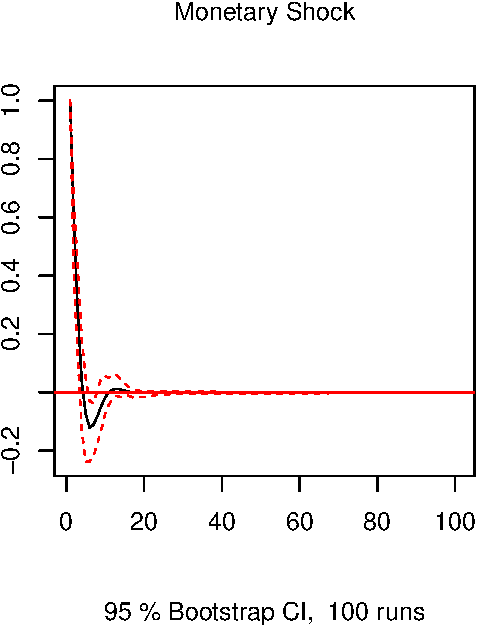
\includegraphics{TS_proj_files/figure-latex/unnamed-chunk-40-3.pdf}

\newpage

Impulse Response of the government consumption to real GDP for each of
the identified shocks:

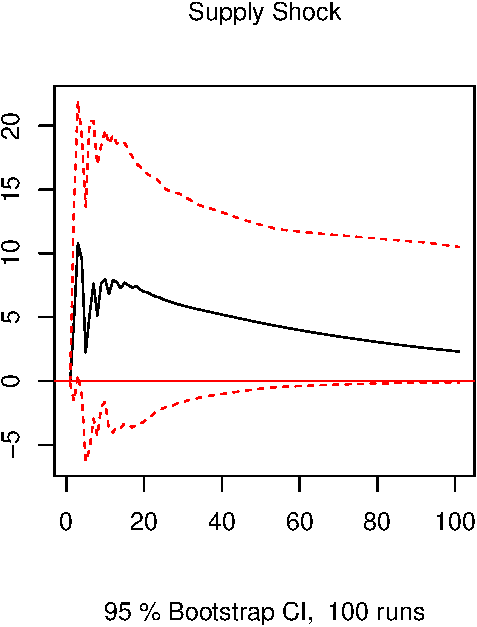
\includegraphics{TS_proj_files/figure-latex/unnamed-chunk-41-1.pdf}
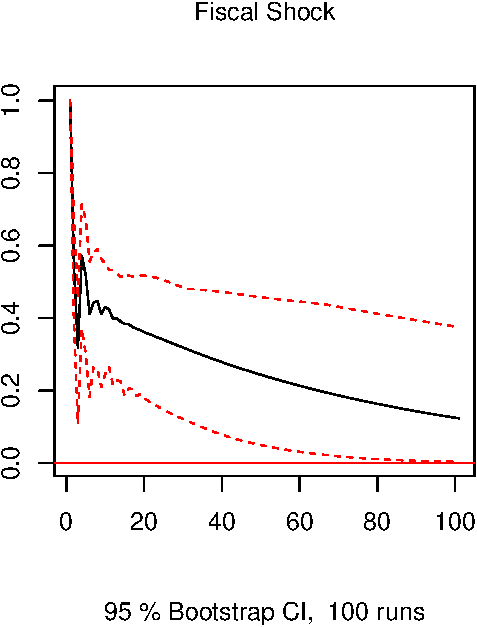
\includegraphics{TS_proj_files/figure-latex/unnamed-chunk-41-2.pdf}
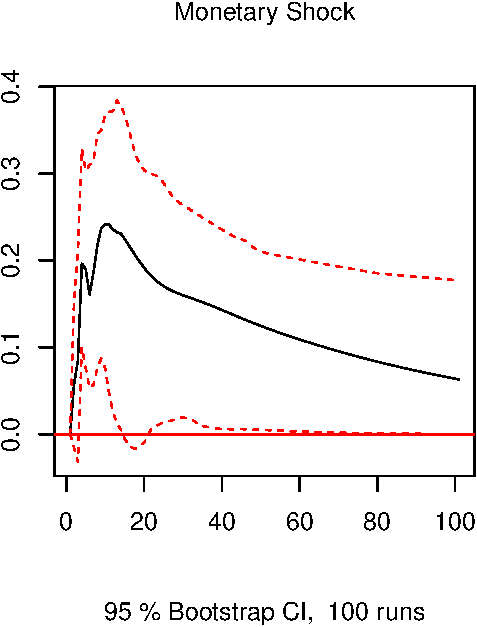
\includegraphics{TS_proj_files/figure-latex/unnamed-chunk-41-3.pdf}

\newpage

Impulse Response of the real GDP for each of the identified shocks:

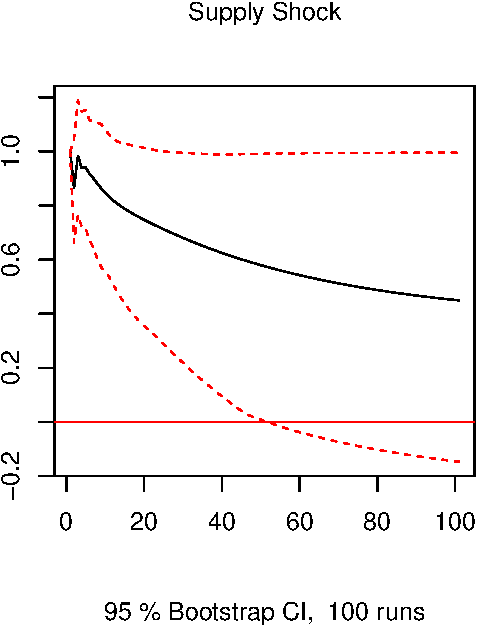
\includegraphics{TS_proj_files/figure-latex/unnamed-chunk-42-1.pdf}
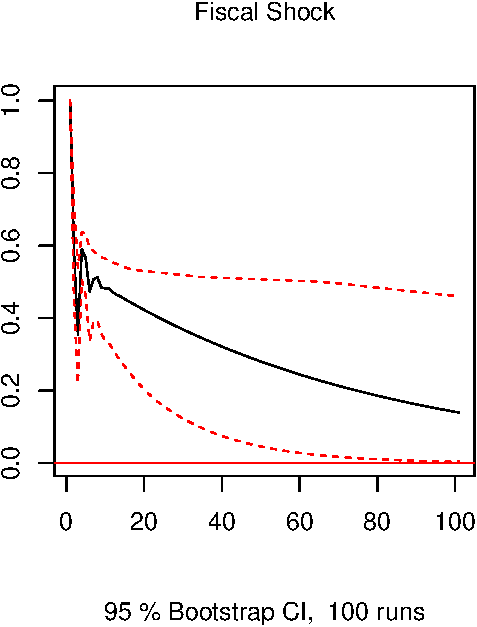
\includegraphics{TS_proj_files/figure-latex/unnamed-chunk-42-2.pdf}
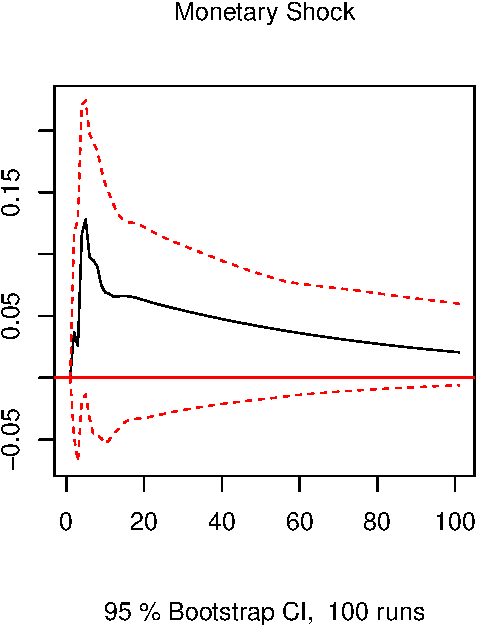
\includegraphics{TS_proj_files/figure-latex/unnamed-chunk-42-3.pdf}

\newpage

Impulse Response of the real interest rate for each of the identified
shocks:

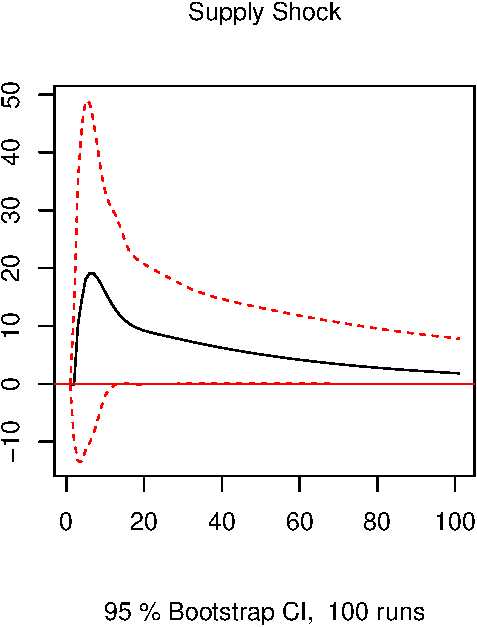
\includegraphics{TS_proj_files/figure-latex/unnamed-chunk-43-1.pdf}
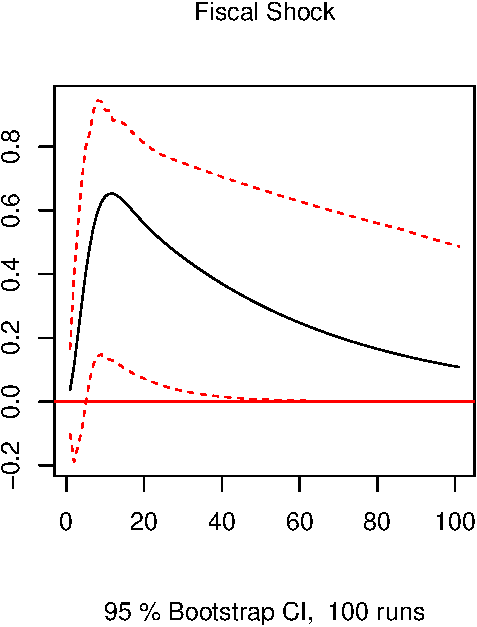
\includegraphics{TS_proj_files/figure-latex/unnamed-chunk-43-2.pdf}
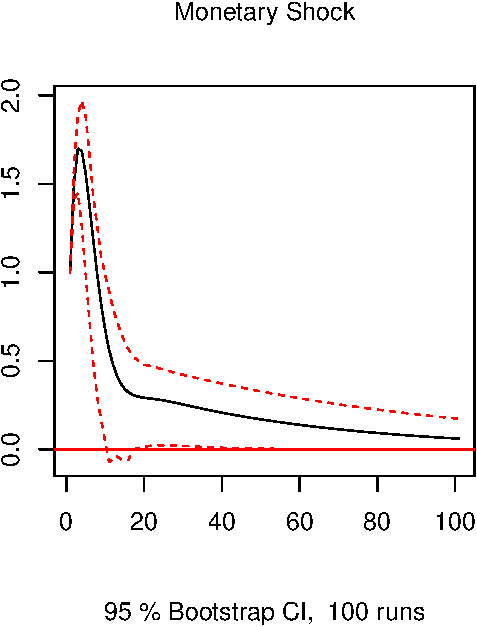
\includegraphics{TS_proj_files/figure-latex/unnamed-chunk-43-3.pdf}

\newpage

Impulse Response of the government consumption to real GDP for each of
the identified shocks:

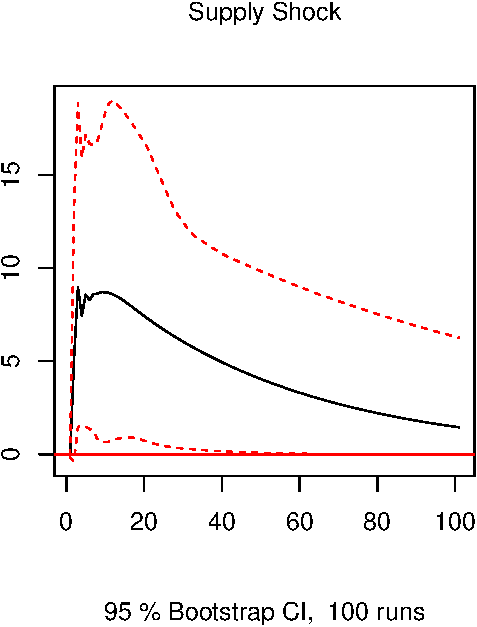
\includegraphics{TS_proj_files/figure-latex/unnamed-chunk-44-1.pdf}
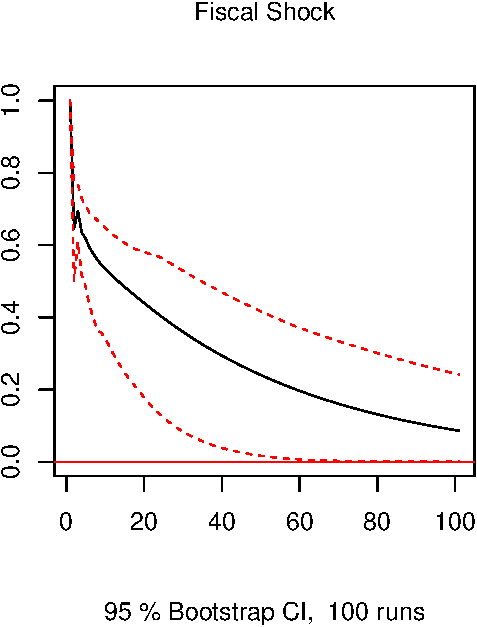
\includegraphics{TS_proj_files/figure-latex/unnamed-chunk-44-2.pdf}
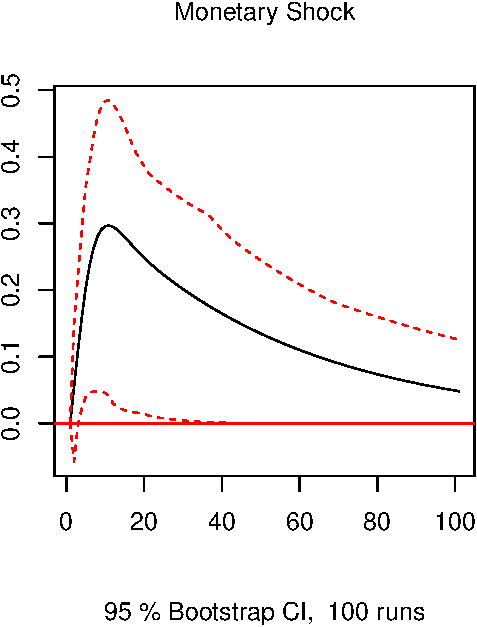
\includegraphics{TS_proj_files/figure-latex/unnamed-chunk-44-3.pdf}

\newpage

\hypertarget{reduced-sample-impulse-response-functions}{%
\subsection{Reduced Sample Impulse Response
Functions}\label{reduced-sample-impulse-response-functions}}

Impulse Response of real GDP for each of the identified shocks:

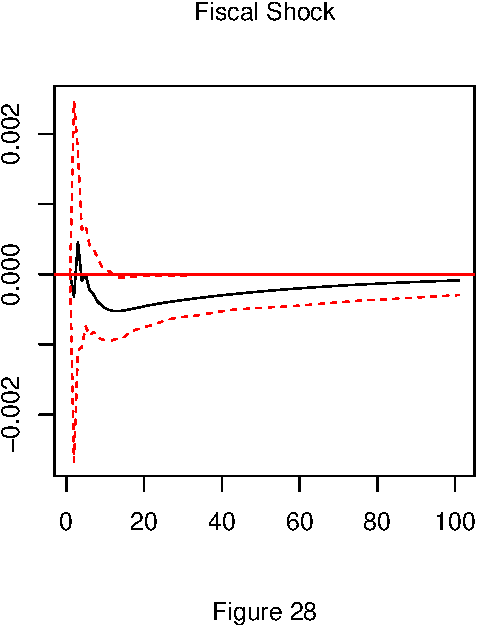
\includegraphics{TS_proj_files/figure-latex/unnamed-chunk-45-1.pdf}
\includegraphics{TS_proj_files/figure-latex/unnamed-chunk-45-2.pdf}
\includegraphics{TS_proj_files/figure-latex/unnamed-chunk-45-3.pdf}
\newpage Impulse Response of the real interest rate for each of the
identified shocks:

\includegraphics{TS_proj_files/figure-latex/unnamed-chunk-46-1.pdf}
\includegraphics{TS_proj_files/figure-latex/unnamed-chunk-46-2.pdf}
\includegraphics{TS_proj_files/figure-latex/unnamed-chunk-46-3.pdf}
\newpage Impulse Response of the government consumption to real GDP for
each of the identified shocks:

\includegraphics{TS_proj_files/figure-latex/unnamed-chunk-47-1.pdf}
\includegraphics{TS_proj_files/figure-latex/unnamed-chunk-47-2.pdf}
\includegraphics{TS_proj_files/figure-latex/unnamed-chunk-47-3.pdf}

\bibliography{Tex/ref}





\end{document}
